\chapter{RESULTS AND DISCUSSION}
The outputs of the program are compared against the output of the software MDLHydroD. The devlopment of the 
MDLHydroD software is explained in \cite{guha2013development} and \cite{guha2015estimation}.
For comparison KCS and KVLCC2 vessels are considered. 

\section{KCS Vessel}
explaination about the input. something something something explaination about the input. something something something
explaination about the input. something something somethingexplaination about the input. something something something
explaination about the input. something something somethingexplaination about the input. something something something
explaination about the input. something something somethingexplaination about the input. something something something

\subsection{Added Mass}
\begin{figure}[!ht]
    \centering
    \begin{subfigure}[b]{0.45\textwidth}
        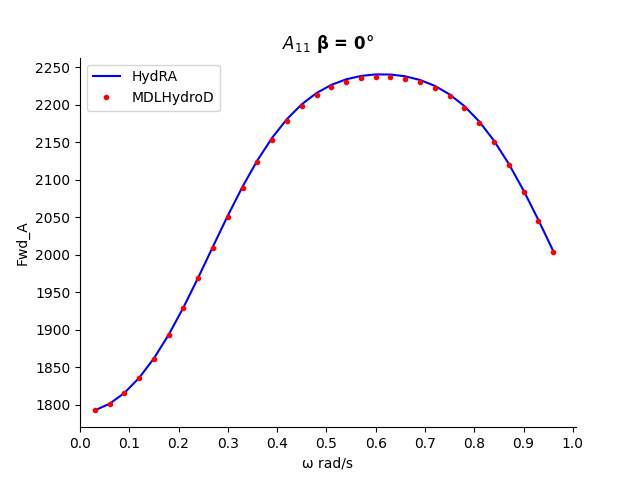
\includegraphics[width=\textwidth]{plots/kcs/added_mass/A11_BETA_0.png}
        \caption{$A_{22} \, \beta = 15^{\circ}$}
    \end{subfigure}
    \begin{subfigure}[b]{0.45\textwidth}
        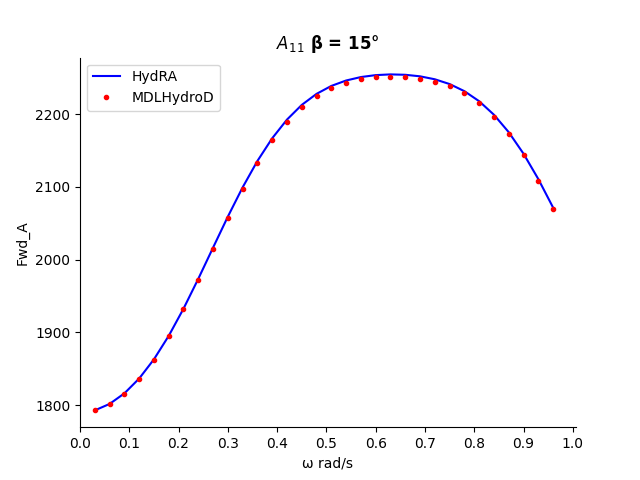
\includegraphics[width=\textwidth]{plots/kcs/added_mass/A11_BETA_15.png}
        \caption{$A_{22} \, \beta = 15^{\circ}$}
    \end{subfigure}
    \caption{KCS vessel added mass comparison - I}
    \label{fig:kcs_addedmass_1}
\end{figure}
\begin{figure}[H]
    \centering
    \ContinuedFloat
    \begin{subfigure}[b]{0.45\textwidth}
        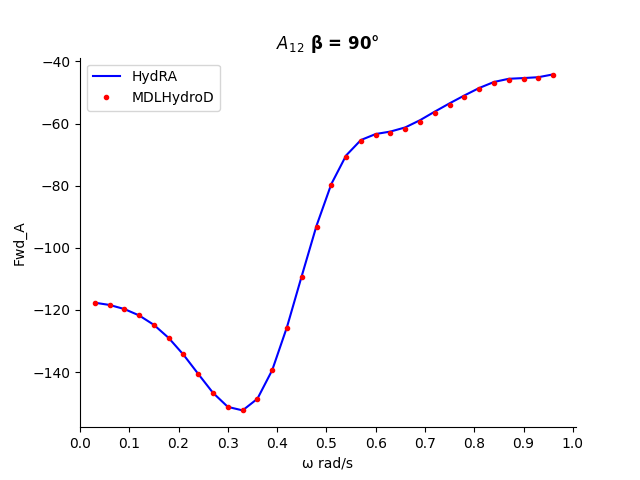
\includegraphics[width=\textwidth]{plots/kcs/added_mass/A12_BETA_90.png}
        \caption{$A_{11}\, \beta=0^{\circ}$}
    \end{subfigure}
    \begin{subfigure}[b]{0.45\textwidth}
        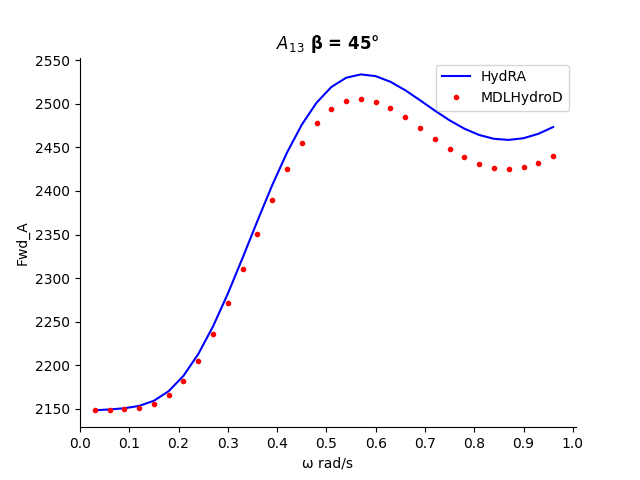
\includegraphics[width=\textwidth]{plots/kcs/added_mass/A13_ BETA_45.png}
        \caption{$A_{22} \, \beta = 11^{\circ}$}
    \end{subfigure}
    \begin{subfigure}[b]{0.45\textwidth}
        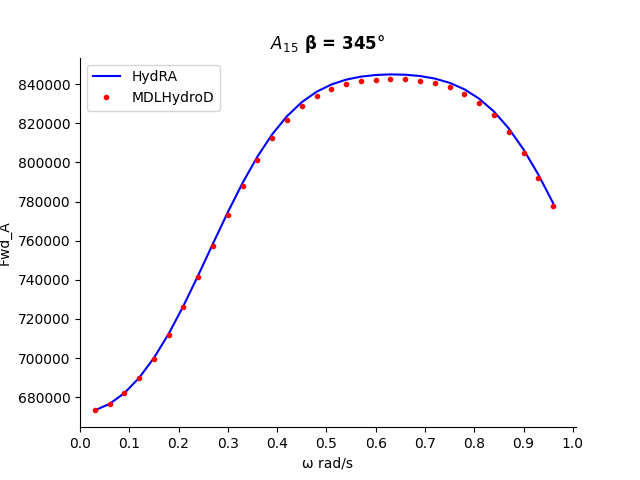
\includegraphics[width=\textwidth]{plots/kcs/added_mass/A15 _BETA_345.png}
        \caption{$A_{22} \, \beta = 12^{\circ}$}
    \end{subfigure}
    \begin{subfigure}[b]{0.45\textwidth}
        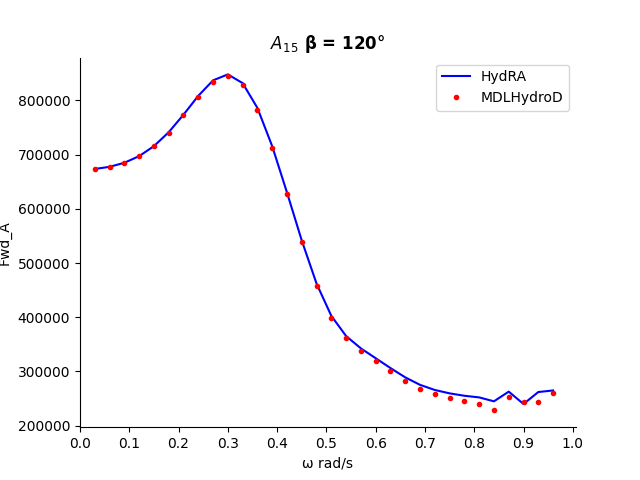
\includegraphics[width=\textwidth]{plots/kcs/added_mass/A15_BETA_120.png}
        \caption{$A_{22} \, \beta = 13^{\circ}$}
    \end{subfigure}
    \begin{subfigure}[b]{0.45\textwidth}
        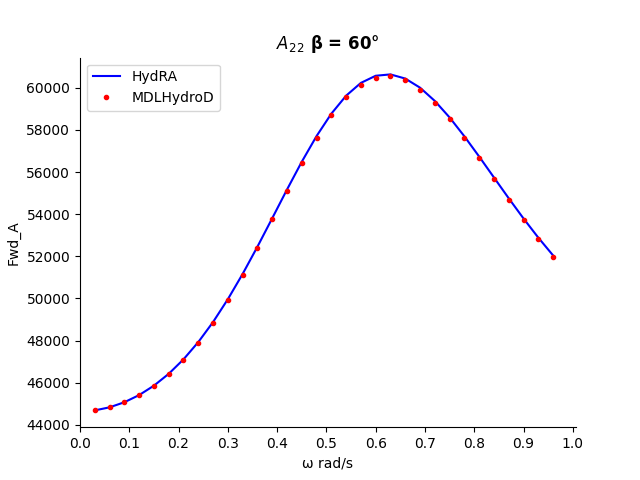
\includegraphics[width=\textwidth]{plots/kcs/added_mass/A22 _BETA_60.png}
        \caption{$A_{22} \, \beta = 14^{\circ}$}
    \end{subfigure}
    \begin{subfigure}[b]{0.45\textwidth}
        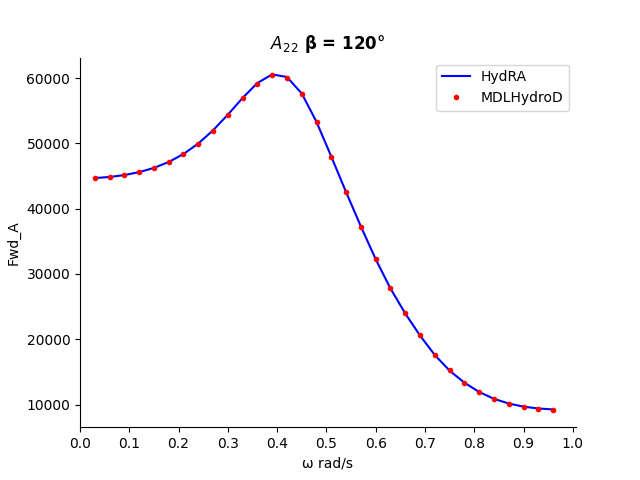
\includegraphics[width=\textwidth]{plots/kcs/added_mass/A22_BETA_120.png}
        \caption{$A_{22} \, \beta = 15^{\circ}$}
    \end{subfigure}
    \begin{subfigure}[b]{0.45\textwidth}
        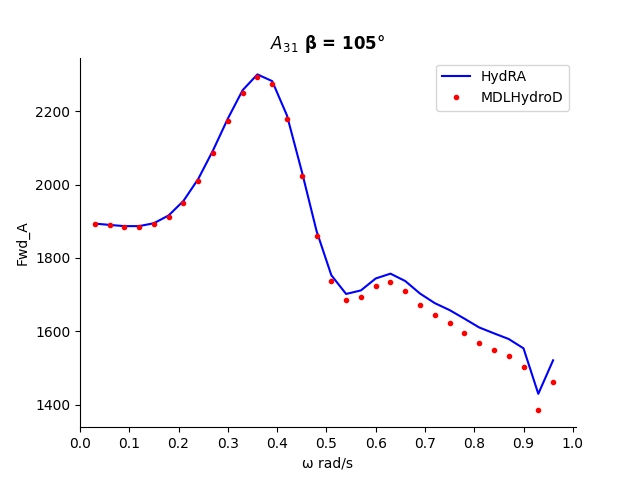
\includegraphics[width=\textwidth]{plots/kcs/added_mass/A31_BETA_105.png}
        \caption{$A_{22} \, \beta = 16^{\circ}$}
    \end{subfigure}
    \begin{subfigure}[b]{0.45\textwidth}
        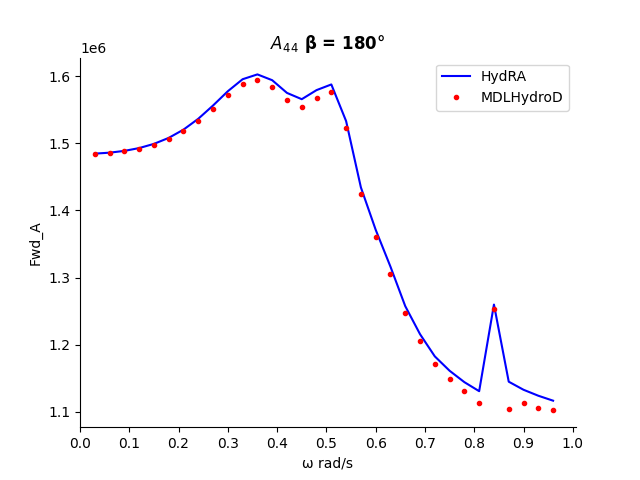
\includegraphics[width=\textwidth]{plots/kcs/added_mass/A44_BETA_180.png}
        \caption{$A_{22} \, \beta = 17^{\circ}$}
    \end{subfigure}
    \caption{KCS vessel added mass comparison - II}
    \label{fig:kcs_addedmass_2}
\end{figure}

\subsection{Radiation Damping}
\begin{figure}[H]
    \centering
    \begin{subfigure}[b]{0.45\textwidth}
        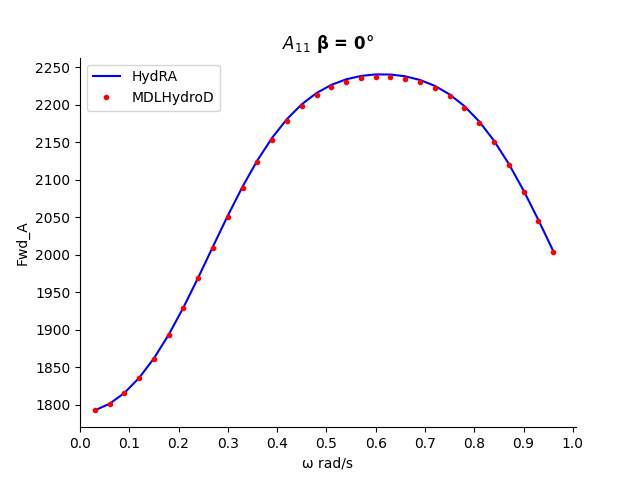
\includegraphics[width=\textwidth]{plots/kcs/added_mass/A11_BETA_0.png}
        \caption{$A_{11}\, \beta=0^{\circ}$}
    \end{subfigure}
    \begin{subfigure}[b]{0.45\textwidth}
        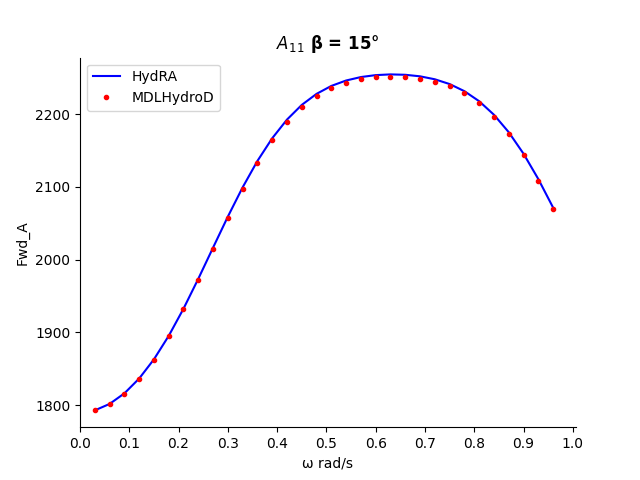
\includegraphics[width=\textwidth]{plots/kcs/added_mass/A11_BETA_15.png}
        \caption{$A_{22} \, \beta = 15^{\circ}$}
    \end{subfigure}
    % \caption{KCS vessel added mass comparison}
    \label{fig:kcs_addedmass_3}
\end{figure}
\subsection{Froude Krylov Force}
\begin{figure}[H]
    \centering
    \begin{subfigure}[b]{0.45\textwidth}
        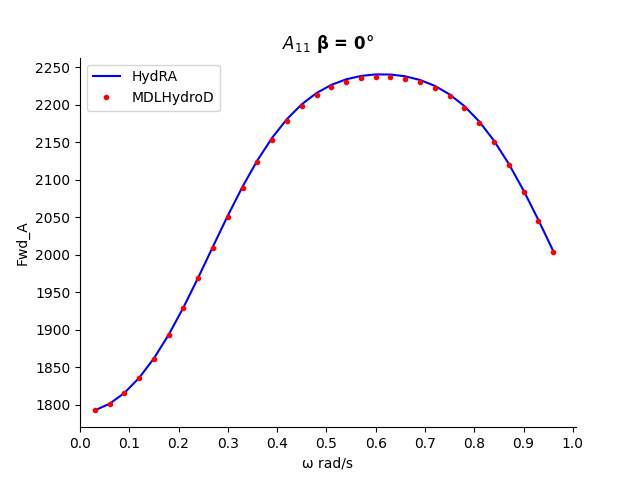
\includegraphics[width=\textwidth]{plots/kcs/added_mass/A11_BETA_0.png}
        \caption{$A_{11}\, \beta=0^{\circ}$}
    \end{subfigure}
    \begin{subfigure}[b]{0.45\textwidth}
        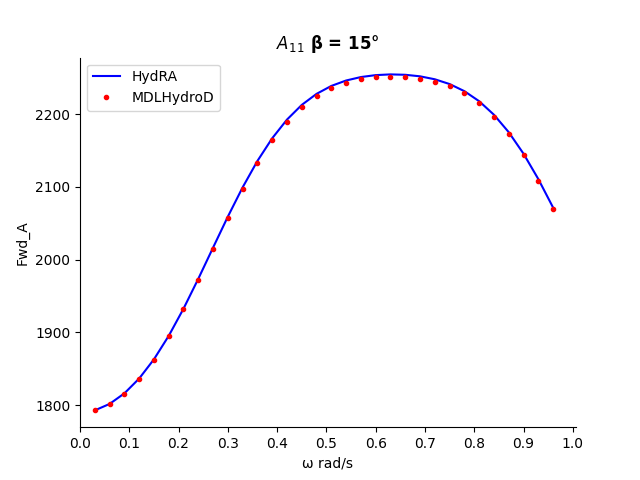
\includegraphics[width=\textwidth]{plots/kcs/added_mass/A11_BETA_15.png}
        \caption{$A_{22} \, \beta = 15^{\circ}$}
    \end{subfigure}
    % \caption{KCS vessel added mass comparison}
    \label{fig:kcs_addedmass_4}
\end{figure}
\subsection{Scattering Force}
\begin{figure}[H]
    \centering
    \begin{subfigure}[b]{0.45\textwidth}
        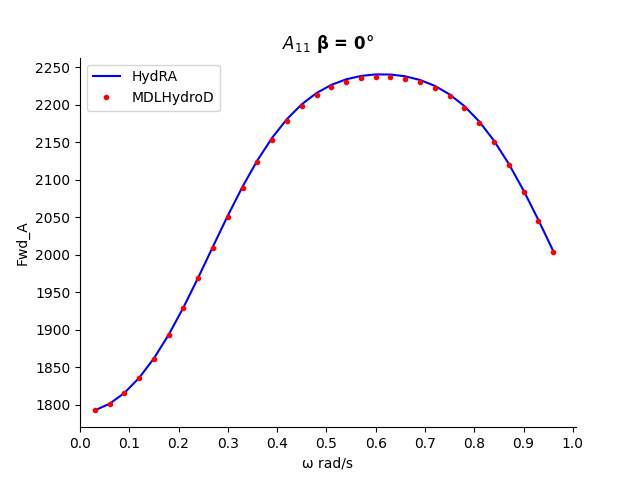
\includegraphics[width=\textwidth]{plots/kcs/added_mass/A11_BETA_0.png}
        \caption{$A_{11}\, \beta=0^{\circ}$}
    \end{subfigure}
    \begin{subfigure}[b]{0.45\textwidth}
        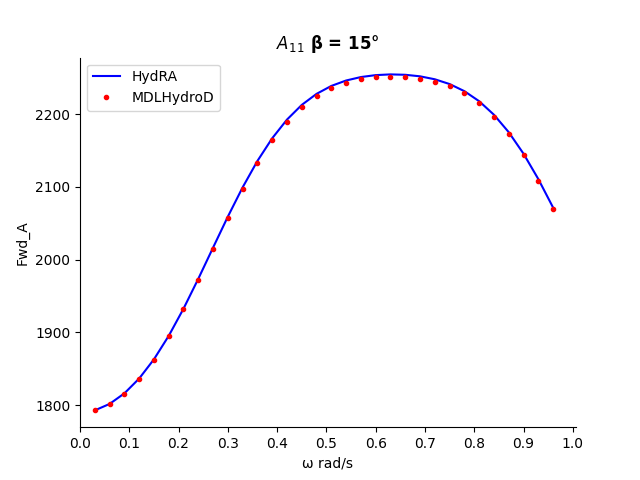
\includegraphics[width=\textwidth]{plots/kcs/added_mass/A11_BETA_15.png}
        \caption{$A_{22} \, \beta = 15^{\circ}$}
    \end{subfigure}
    % \caption{KCS vessel added mass comparison}
    \label{fig:kcs_addedmass_5}
\end{figure}

\section{KVLCC Vessel}
Input parameters for KVLCC2 are given in the following table.
\begin{table}[H]
    \centering
    \begin{tabular}{|c|c|}
        \hline
        parameter & value \\ 
        \hline
        \title{something}
        something & something \\
        something & something \\
        \hline
    \end{tabular}
    \caption{Parameters KCS vessel}
    \label{tab:kvlcc2_inp}
\end{table}